% This is samplepaper.tex, a sample chapter demonstrating the
% LLNCS macro package for Springer Computer Science proceedings;
% Version 2.20 of 2017/10/04
%
\documentclass[runningheads]{llncs}
%
\usepackage{graphicx}
% Used for displaying a sample figure. If possible, figure files should
% be included in EPS format.
%
% If you use the hyperref package, please uncomment the following line
% to display URLs in blue roman font according to Springer's eBook style:
% \renewcommand\UrlFont{\color{blue}\rmfamily}

\begin{document}
%
\title{Contribution Title\thanks{Supported by organization x.}}
%
%\titlerunning{Abbreviated paper title}
% If the paper title is too long for the running head, you can set
% an abbreviated paper title here
%
\author{First Author\inst{1}\orcidID{0000-1111-2222-3333} \and
Second Author\inst{2,3}\orcidID{1111-2222-3333-4444} \and
Third Author\inst{3}\orcidID{2222--3333-4444-5555}}
%
\authorrunning{F. Author et al.}
% First names are abbreviated in the running head.
% If there are more than two authors, 'et al.' is used.
%
\institute{Princeton University, Princeton NJ 08544, USA \and
Springer Heidelberg, Tiergartenstr. 17, 69121 Heidelberg, Germany
\email{lncs@springer.com}\\
\url{http://www.springer.com/gp/computer-science/lncs} \and
ABC Institute, Rupert-Karls-University Heidelberg, Heidelberg, Germany\\
\email{\{abc,lncs\}@uni-heidelberg.de}}
%
\maketitle              % typeset the header of the contribution
%
\begin{abstract}
The abstract should briefly summarize the contents of the paper in
150--250 words.

\keywords{First keyword  \and Second keyword \and Another keyword.}
\end{abstract}
%
%
%




\section{Introduction}
\section{Introduction}
\label{sec:intro}
%SSO的特点
%SSO的现状

As a widely deployed identity management and authentication mechanism in the current Internet, single sign-on (SSO) systems such as OpenID Connect~\cite{OpenIDConnect}, OAuth~\cite{rfc6749} and SAML~\cite{SAML} allow a user to log in to a website, called the \emph{relying party} (RP), using the account registered at another website, called the \emph{identity provider} (IdP). The RPs delegate user authentication to a trusted IdP, who generates \emph{identity proofs} for her visits to these RPs. Thus, the user only needs to remember one credential for the IdP, instead of maintaining different credentials for different RPs.
%        Moreover, SSO shifts the burden of user authentication from RPs to IdPs and reduces security risks and costs at RPs.
SSO has been widely integrated with many application services.
For example, we find that 80\% of the Alexa Top-100 websites support SSO~\cite{Alexa}, and the analysis on the Alexa Top-1M websites identifies 6.30\% with the SSO support~\cite{GhasemisharifRC18}.
Meanwhile, many email and social network providers (such as Google, Facebook, Twitter, etc.) are serving the IdP roles in the Internet. %social identity providers to support social login.


%SSO系统的安全问题,需要保护identity proof的完整性,机密性,绑定性
%完整性:使用公开的为受保护的信息作为identity proof
%机密性:保证由IdP发送给对应的RP,并且传输过程中通道、user agent都是受到保护的
%绑定性:identity proof一定要与对应的RP实现绑定
%SPRESSO中关于impersonation和identity injection的描述。 Authentication is the most fundamental security property of an SSO system. That is, i) an adversary should not be able to log in to an RP, and hence, use the service of the RP, as an honest user, and ii) an adversary should not be able to log in the browser of an honest user under an adversary’s identity (identity injection).
%这段描述两个事情:1.secure authentication 就是能防住impersonation和identity injection。 然而,现在有很多攻击使得这两个无法得到保证。经过分析主要是这三个方面的原因:1)RP接受了未被完整性保护的内容;2)未绑定;3)泄露。
%binding 原文描述 ChenPCTKT14 CCS14 Friendcaster(Friendcaster是一款Facebook的第三方应用,比官方版的功能更加全面) blindly accepting an access token received from a user's device then using this token to exchange for the user's Facebook ID. A malicious application could obtain a legitimate access token from a user, then use this access token to log into Friendcaster as the user. cause they thought Facebook's access tokens were bound to relying parties and checked with every API call: \From Facebook's perspective, the API calls wouldn't appear to be originating from Friendcaster, but the attacker's own app."
%完整性原文描述 IEEE S&P2012~\cite{WangCW12}关于Google问题描述we found that the RPs of Google ID SSO often assume that message fields they require Google to sign would always be signed, which turns out to be a serious misunderstanding (Section 4.1). These problems make us believe that a complete answer to our question can only be found by analyzing SSO schemes on real websites.

% Move to section III
%The primary goal of SSO services is to implement secure user authentication~\cite{SPRESSO}, i.e., to ensure that an honest user can always log in to an honest RP under the correct account. To achieve this, an identity proof generated by the IdP should explicitly specify the authenticated user (i.e., \emph{user identification}) and the RP to which the user attempts to log in (i.e., \emph{receiver designation}). The identify proof should be received only by that RP and user but not by any other entities (i.e., \emph{confidentiality}) and verified by the receiver (i.e., \emph{integrity}). However, various attacks exploit vulnerabilities in different SSO systems to break at least one of these requirements~\cite{ChenPCTKT14, FettKS16,WangCW12,ZhouE14,WangZLG16,YangLLZH16,SomorovskyMSKJ12,MohsenS16}, where the adversaries attempt to either impersonate the victim user at an honest RP or %manipulate the victim user's browser to log in to honest RPs under the adversary's identity. %(i.e., identity injection). For example, Friendcaster was found to accept any received identity proof~\cite{ExplicatingSDK,ChenPCTKT14} (i.e., a violation of receiver designation) so that a malicious RP could log in to Friendcaster as the victim user by replaying the identity proof received from the user to Friendcaster~\cite{MohsenS16}. \cite{WangCW12} reported that some RPs of Google ID SSO accepted user attributes that were not tied to the identity proof (i.e., a potential violation of integrity). As a result, a malicious user could insert arbitrary attributes (e.g., an email address) into the identity proof to impersonate another user at the RP.


%SSO 引入新的隐私问题
%IdP知道用户登录哪个RP
%RP之间可以合谋知道同一个用户登录哪些RP
However, SSO systems have been continuously found vulnerable and insecure~\cite{WangCW12,ccsSunB12,SomorovskyMSKJ12,ArmandoCCCPS13,DiscoveringJCS,dimvaLiM16,WangZLG16,MainkaMS16, MainkaMSW17,YangLCZ18}. Moreover, the adoption of SSO raises a public concern about user privacy~\cite{maler2008venn,NIST2017draft,BrowserID,SPRESSO}, that is whether an adversary is able to track to which RP(s) the user has logged in. 
Unfortunately, almost all the existing SSO protocols leak user privacy in different ways. Take a widely used SSO protocol OpenID Connect (OIDC) as an example. As shown in Fig.~\ref{fig:OpenID}, the login process starts when a user sends a login request to the RP, % (Step 1),
who then constructs a request for identity proof with its identity and redirects the request to the IdP. % (Step 2).
After authenticating the user, the IdP generates an identify proof with the user's and RP's identities, %in Step 4,
which is returned to the user and forwarded to the RP. %in Step 5.
Finally, the RP verifies the identity proof to decide if the user is allowed to log in. In such login instances, by design, an IdP can always see when and where its users log in, in order to generate the identity proof. As a result, a curious IdP can always discover the RPs that a target user has visited over time. This data can be further analyzed to profile users' online activities. Thus, we call this privacy attack \textbf{\em IdP-based login tracing}, which has also been reported by previous research~\cite{BrowserID,SPRESSO}. Similarly, by design, the RPs can learn users' identities from the identify proofs. If the IdP binds an unique or relevant user identifier(s) to identity proofs generated for the same user but different RPs~\cite{Google, FirefoxAccount}, these RPs can collude to correlate the identifier(s) with the user's identity. We denote this privacy risk as \textbf{\em RP-based identity linkage}, which allows the adversaries to not only track the user's online activities but also associate her attributes across multiple RPs by linking her login requests~\cite{maler2008venn}.

As SSO becomes a popular safeguard for various privacy-sensitive web services, the privacy concern is considered more prominent and severe than it was in the past. On one hand, privacy-savvy users may provide no or few personal information to web applications to avoid user tracking or profiling. On the other hand, the use of popular SSO services such as Google Account opens a door for IdPs and application providers to recover users' online traces and profiles, which makes users' privacy protection effort in vain. Several large IdPs, especially the social IdPs, are known to be interested in collecting users' online behavioral data for various purposes (e.g., Screenwise Meter~\cite{googlenews} and Onavo~\cite{Onavo}). Serving the IdP role makes it possible for them to collect such information. Meanwhile, service providers hosting multiple web applications take an advantaged position to correlate users' multiple logins at different RPs through internal information integration. Finally, privacy-preserving record linkage~\cite{agrawal2003information} and private set intersection~\cite{de2010practical} technologies allow multiple RPs to share data without violating their clients' privacy, which pave the path for cross-organizational RP-based identity linkage.

																																																																																																																																																																																																																																																																																																																																																																																																																																																																																																																																																																																																																																																																																																																																																																																																																																			
%also raises privacy concerns regarding online user tracking and profiling.
%Imagine that, a user concerning her privacy would avoid to leave her full sensitive information at an application. The user may use multiple web applications and only leave parts of her sensitive messages at each applications, for example, using  real name on social website, the address on shopping website and the phone number on Telecom website. And she would try not to leave any linkable message to avoid applications combining her informations, for example, if she leave the email on each applications, they can combine the parts of informations through the email. However,  the privacy leaks in SSO systems make her effort in vain. As long as a user employs the SSO system, such as Google Account, to log in to these applications, the applications providers and Google can combine your informations based on the SSO account.

%google and facebook的负面新闻
%1. service provider(如DNS)知道你访问了,可以带来很多问题。但是还是不同的,DNS里profile需要评估的是two behavior vectors的similarities,而IdP中都不需要,因为IdP能够区分two behavior vectors 是否来自相同节点。

Several solutions have been proposed to protect user privacy in SSO login~\cite{maler2008venn,NIST2017draft,BrowserID,SPRESSO}. However, to the best of our knowledge, none of them provides a comprehensive protection to defend against IdP-based login tracing and RP-based identity linkage {\em at the same time}. For example, as recommended by NIST~\cite{NIST2017draft} and specified in several SSO protocols~\cite{OpenIDConnect, SAMLIdentifier}, pairwise pseudonymous identifier (PPID) is generated by the IdP to identify a user to an RP, which cannot be correlated with the user's PPID at another RP. Thus, collusive RPs cannot link a user's logins from her PPIDs. However, PPID-based approaches cannot prevent IdP-based login tracing, since the IdP needs to know which RP the user visits in order to generate the correct identify proof. On the contrary, BrowserID~\cite{BrowserID} and SPRESSO~\cite{SPRESSO} were proposed to defend against IdP-based login tracing. However, both solutions are vulnerable to RP-based identity linkage. In BrowserID (and its prototypes known as Mozilla Persona~\cite{persona} and Firefox Accounts~\cite{FirefoxAccount}), the IdP does not know the identity of the requesting RP. Instead, it generates a special ``identity proof'' to bind the user's unique identifier (e.g., email address) to a public key, so that the user can sign another subsidiary identity proof to bind her identity with the RP's identity and send both identity proofs to the RP. Obviously, when a user logs in to different RPs, the RPs can extract a same user identifier from different identity proofs and correlate these logins. In SPRESSO, the RP creates a one-time pseudo-identifier in each login. Then, the IdP generates an identity proof binding this pseudo-identifier and the user's identity (i.e., email address). %and returns it through a trusted third-party entity called forwarder.
Similarly, the RPs can correlate a user's logins using her unique identifier in the identity proofs.

Recently more and more IdPs have been considering the user's privacy serious. For example, one of the most worldwide popular instant messaging applications, WeChat, also working as the IdP service provider, enables a user to create different  plain accounts for login on multiple RPs, shown in Figure~\ref{fig:wechat}.  Moreover,  Active Directory Federation Services and Oracle Access Management support the use of PPID~\cite{MS, Oracle}; identity service providers such as NORDIC APIS and CURITY suggest adopting PPID in SSO to protect user privacy~\cite{Nordic, Curity}.

Unfortunately, the techniques proposed by previous research cannot be directly integrated to address the two major types of privacy risks in SSO at the same time. In fact, it requires a non-trivial redesign of the SSO system to defend against IdP-based login tracing and RP-based identity linkage while providing a secure and compatible SSO service. In this paper, we first conceptualize the privacy problem in SSO as {\em an identifier transformation problem} and explain the reasons that limit existing solutions from fully protecting user privacy against curious IdPs and collusive RPs. Based on our analysis, we propose an Unlinkable Privacy-PREserving Single Sign-On (UPPRESSO) system to provide a comprehensive protection against both types of privacy attacks.

UPPRESSO designs three one-way identifier-transformation functions based on elliptic curve cryptography. Using the one-way trapdoor function $\mathcal{F}_{ID_{RP} \mapsto PID_{RP}}(ID_{RP}, T)$, the RP converts its identity $ID_{RP}$ into a privacy-preserving pseudo-identifier $PID_{RP}$ based on a randomly selected trapdoor $T$. Similarly, the IdP uses the one-way function  $\mathcal{F}_{ID_{U} \mapsto PID_{U}}(ID_U, PID_{RP})$ to generate a privacy-preserving pseudo-identifier $PID_U$ for the user based on her identity $ID_U$ and $PID_{RP}$. Finally, using a special identifier-transformation function $\mathcal{F}_{PID_{U} \mapsto Account}(PID_U, PID_{RP}, T)$, the RP is able to map all the different privacy-preserving pseudo-identifiers of a user, which are created in her different login sessions to that RP, to a same $Account$ that identifies the user to the RP. The three identifier-transformation functions work cooperatively to ensure: (\emph{a}) when a user logs in to an RP multiple times, the RP can always map $PID_U$s to a unique $Account$ without knowing the user's identity $ID_U$; moreover, when a user logs in to multiple RPs, (\emph{b}) a curious IdP learns nothing about the identities of these RPs from $PID_{RP}$s, and (\emph{c}) collusive RPs cannot link $PID_U$s to a particular user %or associate them together,
(\emph{d}) nor correlate $Account$s of a same user at different RPs.
We summarize our contributions as follows.
%我们的贡献
%提出协议
%考虑能否根据模型进行分析
%实现原型系统
%The main contributions of UPPRESSO are as follows:
\begin{itemize}
\vspace{-\topsep}
\item We are among the first to conceptualize the privacy problem in SSO as an identifier-transformation problem and analyze the strengths and limitations of existing SSO privacy protection solutions.
\vspace{-\topsep}
\item We propose a comprehensive solution to hide the users' login traces from curious IdPs and collusive RPs. To the best of our knowledge, UPPRESSO is the first SSO system that secures SSO services against IdP-based login tracing and RP-based identity linkage.
\vspace{-\topsep}
\item We provide the reduction from UPPRESSO scheme to DDH Assumption proving that it is protected from IdP-based login tracing and RP-based identity linkage,
and analyze the security of UPPRESSO based on a formal model of the web infrastructure and formally prove that it provides satisfying security properties.
\vspace{-\topsep}
\item We implement a prototype of UPPRESSO based on an open-source implementation of OIDC, which requires only small modifications to support three identifier-transformation functions for privacy protections. Thus, UPPRESSO is compatible with existing SSO systems. Moreover, our prototype leverages HTML 5 features in the implementation so that it can be used across platforms (e.g., PCs, smart phones and other devices). %Unlike  BrowserID and SPRESSO,  does not require non-trivial re-designs of SSO services, which makes it more .
\vspace{-\topsep}
\item We compare the performance of the UPPRESSO prototype with the state-of-the-art SSO systems (i.e., OIDC~\cite{OpenIDConnect} and SPRESSO~\cite{SPRESSO}) and demonstrate its efficiency.
\end{itemize}
\vspace{-\topsep}
%文章结构
The rest of the paper is organized as follows. We first introduce the background and preliminaries in Section~\ref{sec:background}. Then, we describe the identifier-transformation-based approach and the threat model in Sections~\ref{sec:challenge} and \ref{sec:assumptionandthreatmodel}. Section \ref{sec:UPPRESSO} presents the details of our UPPRESSO design, followed by a formal analysis of its privacy and security in Section~\ref{sec:privacy} and ~\ref{sec:formal}. We explain the implementation specifics and experiment evaluation in Section~\ref{sec:implementation}, discuss the extensions and related works in Section~\ref{sec:discussion} and~\ref{sec:related}, and conclude our work in Section~\ref{sec:conclusion}.






\section{First Section}
\subsection{A Subsection Sample}
Please note that the first paragraph of a section or subsection is
not indented. The first paragraph that follows a table, figure,
equation etc. does not need an indent, either.

Subsequent paragraphs, however, are indented.

\subsubsection{Sample Heading (Third Level)} Only two levels of
headings should be numbered. Lower level headings remain unnumbered;
they are formatted as run-in headings.

\paragraph{Sample Heading (Fourth Level)}
The contribution should contain no more than four levels of
headings. Table~\ref{tab1} gives a summary of all heading levels.

\begin{table}
\caption{Table captions should be placed above the
tables.}\label{tab1}
\begin{tabular}{|l|l|l|}
\hline
Heading level &  Example & Font size and style\\
\hline
Title (centered) &  {\Large\bfseries Lecture Notes} & 14 point, bold\\
1st-level heading &  {\large\bfseries 1 Introduction} & 12 point, bold\\
2nd-level heading & {\bfseries 2.1 Printing Area} & 10 point, bold\\
3rd-level heading & {\bfseries Run-in Heading in Bold.} Text follows & 10 point, bold\\
4th-level heading & {\itshape Lowest Level Heading.} Text follows & 10 point, italic\\
\hline
\end{tabular}
\end{table}


\noindent Displayed equations are centered and set on a separate
line.
\begin{equation}
x + y = z
\end{equation}
Please try to avoid rasterized images for line-art diagrams and
schemas. Whenever possible, use vector graphics instead (see
Fig.~\ref{fig1}).

\begin{figure}
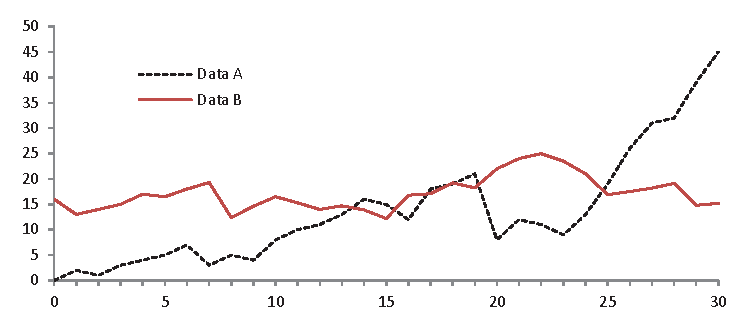
\includegraphics[width=\textwidth]{fig1.eps}
\caption{A figure caption is always placed below the illustration.
Please note that short captions are centered, while long ones are
justified by the macro package automatically.} \label{fig1}
\end{figure}

\begin{theorem}
This is a sample theorem. The run-in heading is set in bold, while
the following text appears in italics. Definitions, lemmas,
propositions, and corollaries are styled the same way.
\end{theorem}
%
% the environments 'definition', 'lemma', 'proposition', 'corollary',
% 'remark', and 'example' are defined in the LLNCS documentclass as well.
%
\begin{proof}
Proofs, examples, and remarks have the initial word in italics,
while the following text appears in normal font.
\end{proof}
For citations of references, we prefer the use of square brackets
and consecutive numbers. Citations using labels or the author/year
convention are also acceptable. The following bibliography provides
a sample reference list with entries for journal
articles~\cite{ref_article1}, an LNCS chapter~\cite{ref_lncs1}, a
book~\cite{ref_book1}, proceedings without editors~\cite{ref_proc1},
and a homepage~\cite{ref_url1}. Multiple citations are grouped
\cite{ref_article1,ref_lncs1,ref_book1},
\cite{ref_article1,ref_book1,ref_proc1,ref_url1}.
%
% ---- Bibliography ----
%
% BibTeX users should specify bibliography style 'splncs04'.
% References will then be sorted and formatted in the correct style.
%
% \bibliographystyle{splncs04}
% \bibliography{mybibliography}
%
\begin{thebibliography}{8}
\bibitem{ref_article1}
Author, F.: Article title. Journal \textbf{2}(5), 99--110 (2016)

\bibitem{ref_lncs1}
Author, F., Author, S.: Title of a proceedings paper. In: Editor,
F., Editor, S. (eds.) CONFERENCE 2016, LNCS, vol. 9999, pp. 1--13.
Springer, Heidelberg (2016). \doi{10.10007/1234567890}

\bibitem{ref_book1}
Author, F., Author, S., Author, T.: Book title. 2nd edn. Publisher,
Location (1999)

\bibitem{ref_proc1}
Author, A.-B.: Contribution title. In: 9th International Proceedings
on Proceedings, pp. 1--2. Publisher, Location (2010)

\bibitem{ref_url1}
LNCS Homepage, \url{http://www.springer.com/lncs}. Last accessed 4
Oct 2017
\end{thebibliography}
\end{document}
